\section{Auswertung}
\label{sec:Auswertung}

Wurde im Folgenden ein Versuch ohne Dancerarm durchgeführt, so wurde der Draht direkt über das Kugellager der darunter liegenden Leiste geführt. Des weiteren gilt für alle folgenden Graphiken, dass die Unsicherheitsbalken stets die einfache Standardabweichung angebegen.\newline
Wickelt man die selbe Wicklung, auf der Spule $SP_K$, zweimal mit unterschiedlicher Geschwindigkeit, so wird der, bereits in \autoref{sec:Physikalisches Modell} erwähnte, Effekt einer geschwindigkeitsabhängigen Drahtspannung , bzw. Rückstellkraft $F_R$ sichtbar. Der Versuch wurde je einmal mit Dancerarm und einmal ohne Dancerarm durchgeführt.

\begin{figure}[H]
    \centering
    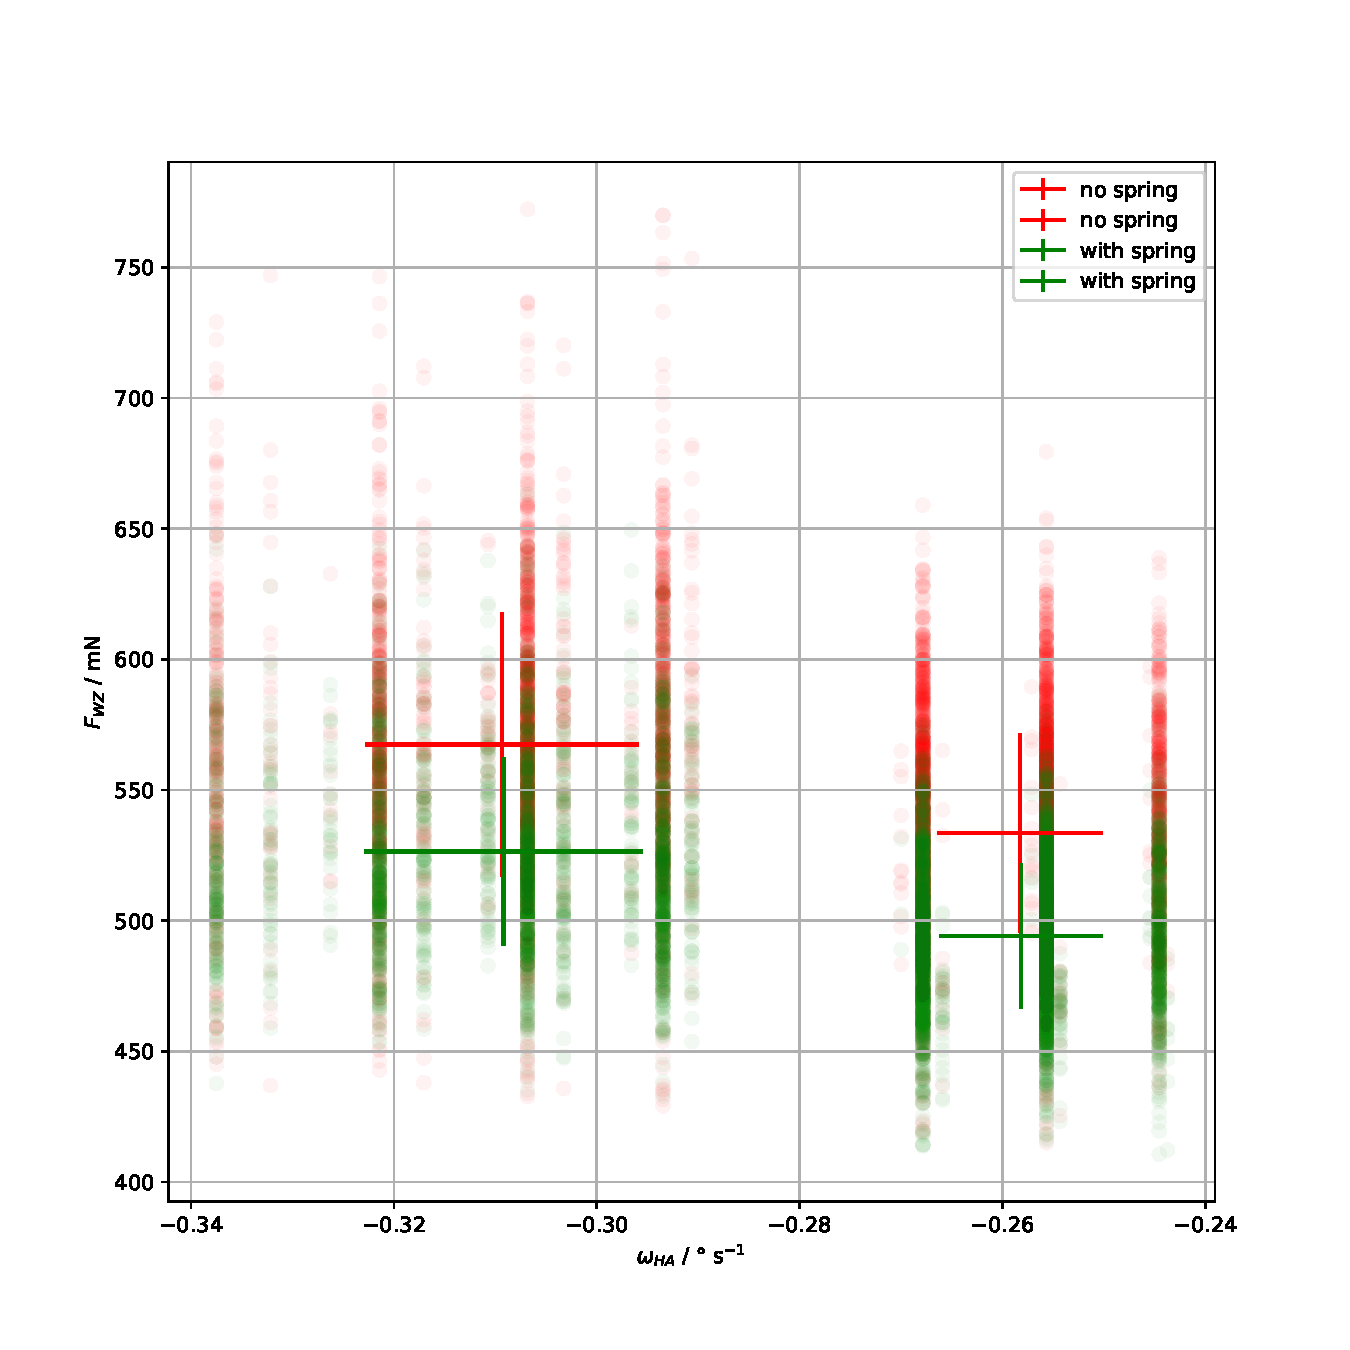
\includegraphics[width=0.9\textwidth]{./const_speed.pdf}
    \caption{Darstellung der an der Wägezelle gemessenen Kraft während einer Wickelphase mit vorgegebener, konstanter Geschwindigkeit, $F_{WZ}$ in Abhängigkeit von der Winkelgeschwindigkeit der Hauptachse $\omega_{HA}$. Die, mit Unsicherheitsbalken versehenen, vier Datenpunkte beschreiben jeweils das arithmetische Mittel des angegeben Größe.}
    \label{fig:plot_const_speed}
\end{figure}


Eine mögliche Erklärung für die, in siehe \autoref{fig:plot_const_speed} ersichtliche, Geschwindigkeitsabhängigkeit der Drahtspannungskraft $\tau(v)$, bzw. Rückstellkraft $F_R(v)$, wäre, dass irgendwo im System eine Geschwindigkeitsabhängige Reibung vorkommt.
Geschwindigkeitsabhängige Reibungskräfte sind zum beispiel in der Aerodynamik als Luftwiderstand bekannt.
Unsere Annahme ist daher, dass entweder die Reibung, die durch das Öl in den V-Nut Kugellagern entsteht relativ groß ist, oder was wahrscheinlicher ist, dass die Reibungskraft des Filzes geschwindigkeitsabhängig ist.
Dies wiederum erklärten wir uns durch die Rückstellkräfte einzelner Filzfaser, die ähnlich auf den Faden drücken wie Fahrtwinddruck auf ein Auto.



Für den nächsten Versuch wurden die selbe Wicklung, bei gleichbleibenden Wickelparametern, einmal mit Dancerarm und einmal ohne, je für beide Spulenkörper, durchgeführt. Da die Zeit zwischen zwei Messwerten nicht konstant ist, sondern leicht schwankt (für Erklärung siehe \autoref{sec:Messschleife}), wurden die Daten Interpoliert, um äquidistante Messwertschritte zu erhalten. Danach wurde jeweils eine Fast-Fourier-Transformation $FFT$ durchgeführt und das Ergebnis in \autoref{fig:ffts} dargestellt.

\begin{figure}[H]
    \centering
    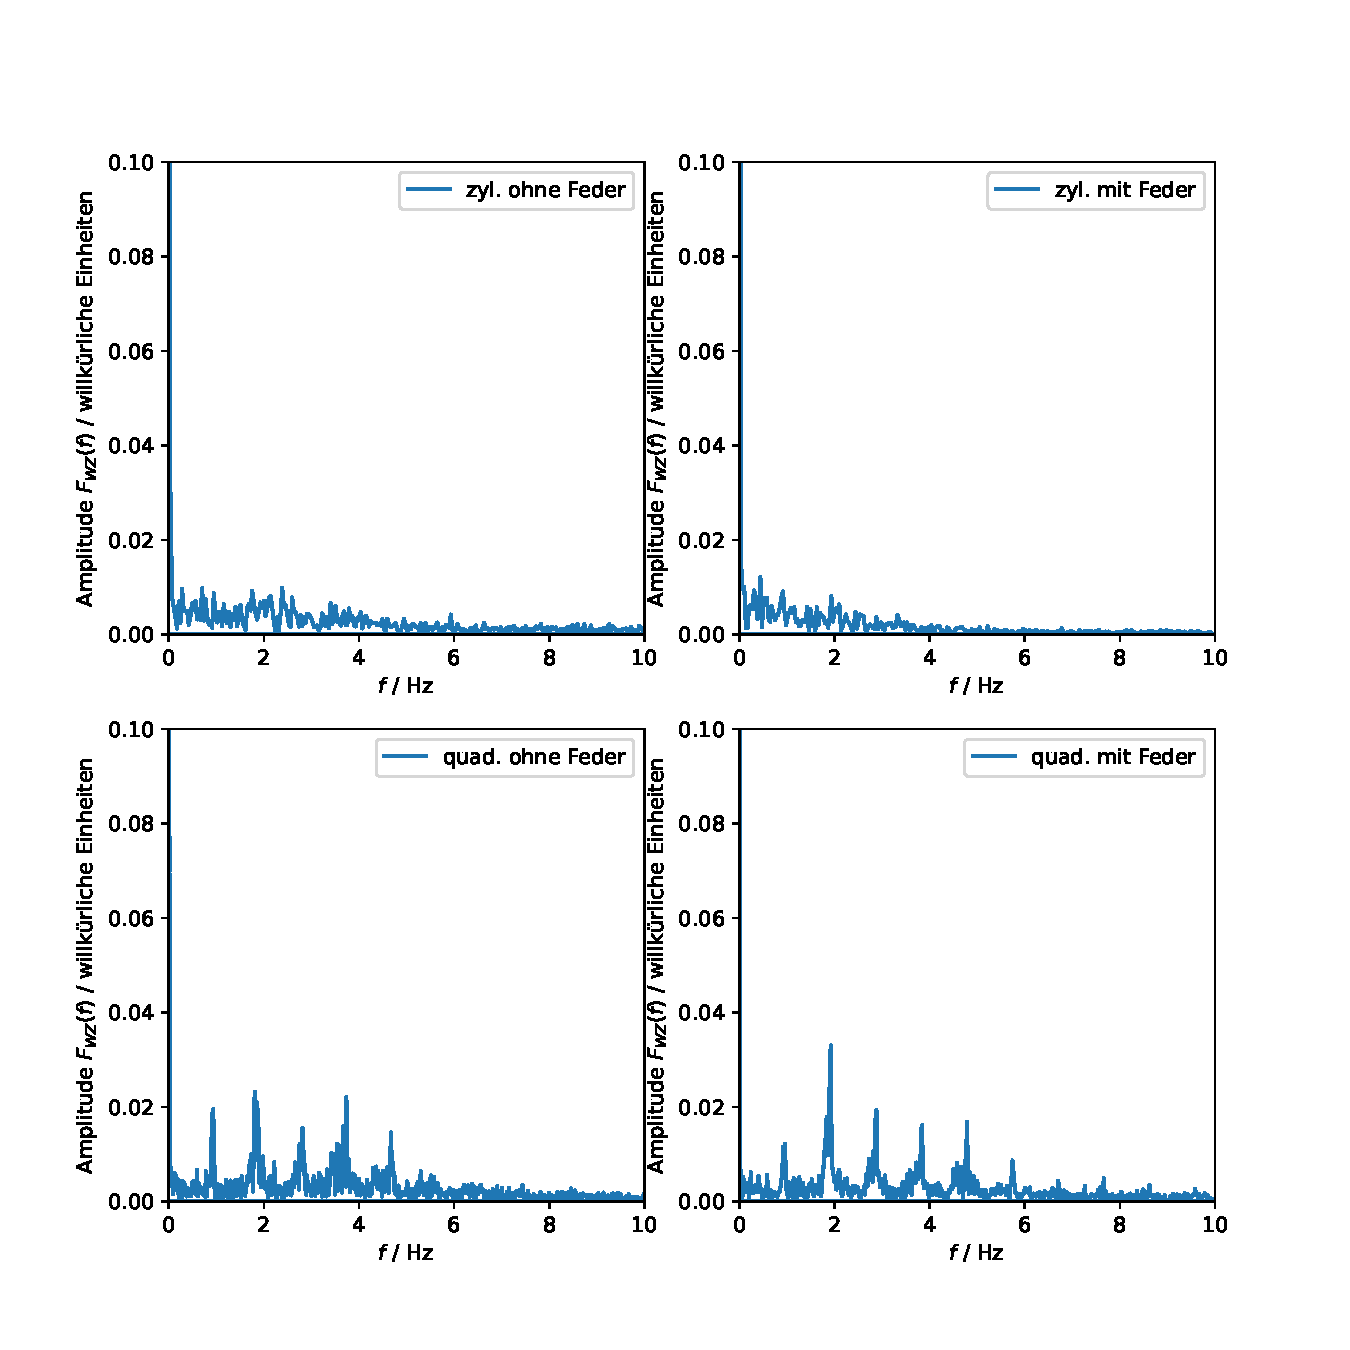
\includegraphics[width=0.9\textwidth]{./ffts.pdf}
    \caption{Darstellung der $FFTs$ für beide Spulenkörper, je einmal ohne Dancerarm und einmal mit Arm}
    \label{fig:ffts}
\end{figure}

Betrachtet man die zwei, $SP_K$, zugehörigen Graphen, in \autoref{fig:ffts}, so sieht man, dass es keinen signifikanten Unterschied gibt wenn der Dancerarm nicht verwendet wird.
Der Einfluss der, in \autoref{sec:Physikalisches Modell} vermuteten, abklingenden Schwingung, angeregt durch den Wechsel von Haft- zu Gleitreibung, scheint vergleichsweise wenig Einfluss auf die Schwingung der Drahtspannung zu haben.
Sieht man sich hingegen die zwei Graphen von $SP_Q$ an, so fallen sofort die deutlichen Peaks in der $FFT$ auf  welche auf das periodische Schwingen der Drahtspannung hindeuten.

Die Peaks bei ca. 1 Hz ist auf die Unwuchtigkeit der Hauptachse, der bei ca. 4 Hz Auf die 4 Ecken des Spulenkörpers zurückzuführen.
Bei den restlichen Peaks dürfte es sich um Obertöne handeln, welche ganzzahlige vielfache der Grundfrequenz 1 Hz sind.

Zur Untersuchung der Start-, bzw. Abbremsphasen eines Wickeldurchganges sind in \autoref{fig:plot_beschleunigung} die zwei Phasen, je für beide Spulentypen dargestellt. Die Messungen wurde jeweils mit der selben Beschleunigung und Endgeschwindigkeit durchgeführt.


\begin{figure}[H]
    \centering
    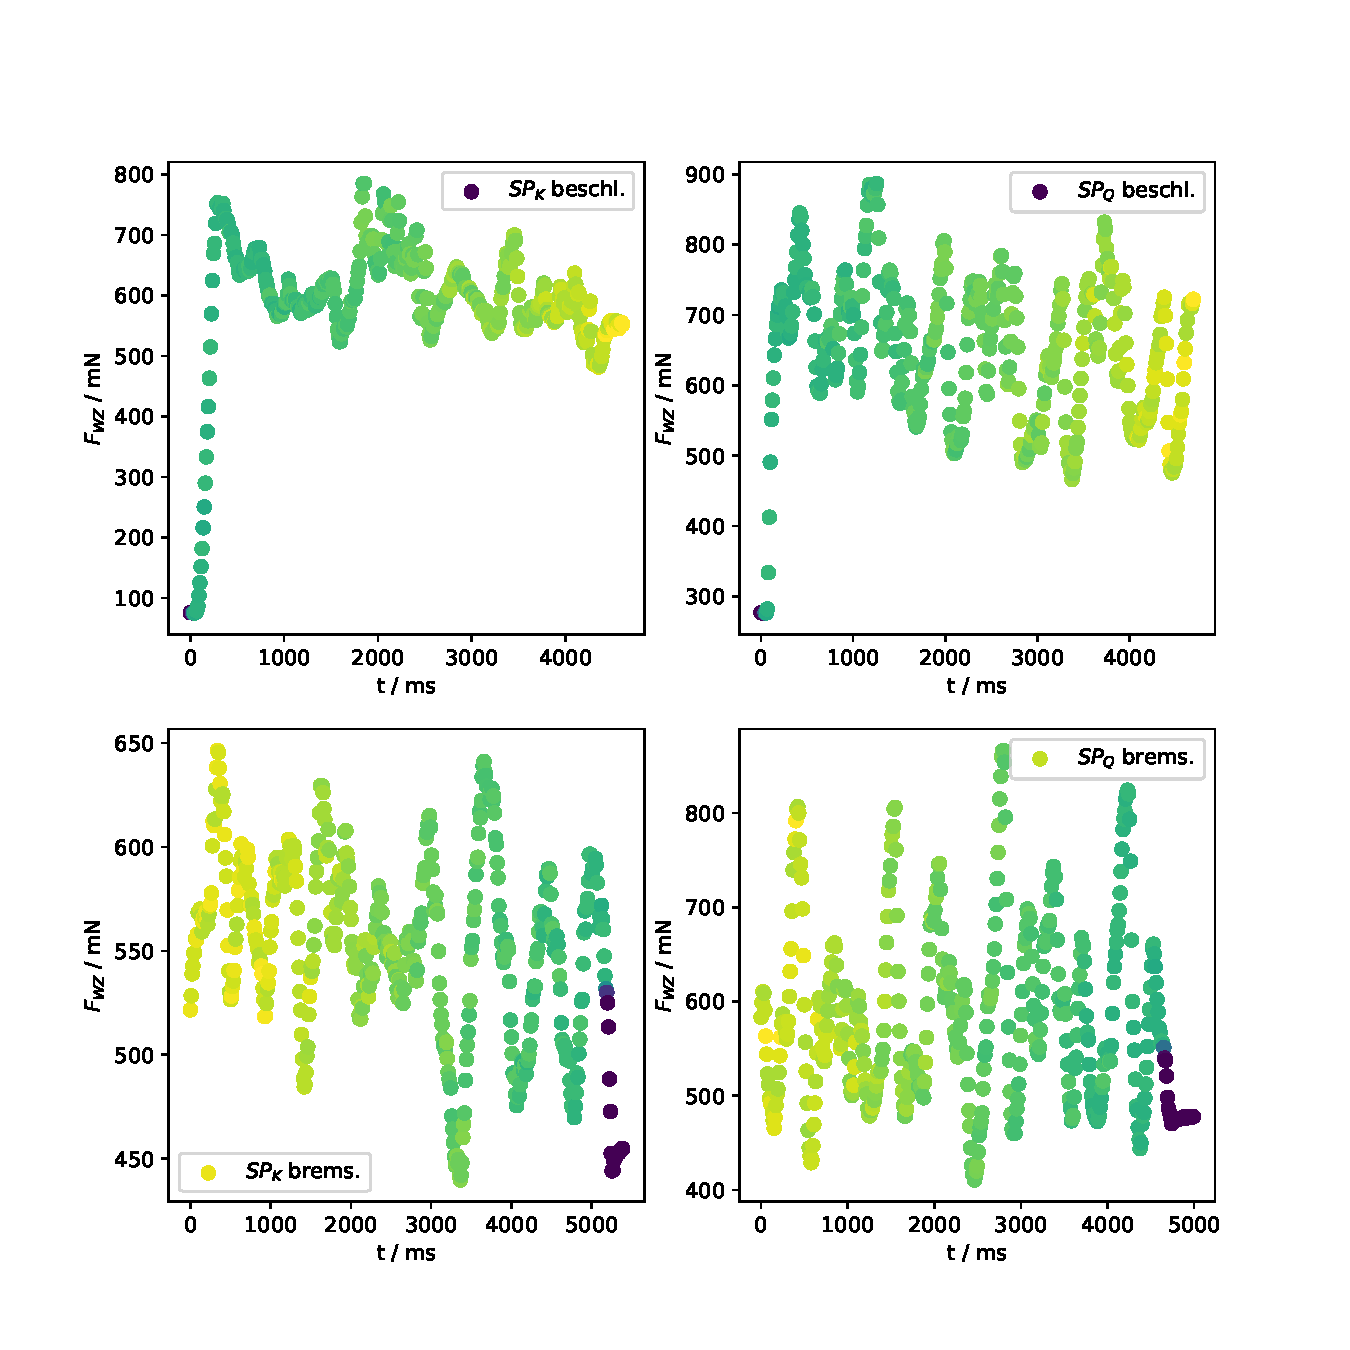
\includegraphics[width=0.9\textwidth]{./besch.pdf}
    \caption{Darstellung der an der Wägezelle gemessenen Kraft $F_{WZ}$ gegen die Zeit $t$. Die Farbcodierung stellt die Geschwindigkeit der HA $\omega_{HA}$, von Gelb (große Geschwindigkeit) bis Lila (kleine Geschwindigkeit), dar. Für alle vier Graphen wurden die selben Wickelparameter verwendet. Die Messungen fanden ohne Dancerarm statt.}
    \label{fig:plot_beschleunigung}
\end{figure}

Sieht man sich die Graphiken der Bremsphasen an, so fällt auf, dass das System stark gedämpft ist. Betrachtet man die lilafärbigen Teile des Datensatzes, so sieht man nur einen relativen kleinen trägheitsbedingten Ausschwung der Kraft unter die anschließende Ruhelage. Die Filzklemme scheint also ihre im Modell (siehe \autoref{sec:Physikalisches Modell}) angedachte Funktion gut zu erfüllen. Im Bezug auf die Beschleunigungsphasen ist anzumerken, dass das die Kraft sehr schnell anfängt um einen Wert herum zu schwanken, obwohl die Beschleunigungsphase immer noch anhält. Dies wurde von uns ebenfalls nicht erwartet, da hier mit einer konstanten Beschleunigung gearbeitet wurde.  



